\documentclass[11pt]{beamer}
\mode<presentation>
%\documentclass[handout,compress]{beamer}
\usepackage{beamerthemedefault}
\usepackage{graphicx}
\usepackage{hyperref}
\usepackage{subfigure}
\usepackage{color}
\usepackage{multicol}
\usepackage{bm} 
\usepackage{tikz}
\usepackage{listliketab}

\usetheme{CambridgeUS}
\makeatletter
\makeatother
\usetikzlibrary{shapes,backgrounds}
\tikzstyle{cblue}=[circle, draw, thin,fill=cyan!20, scale=0.8]
\tikzstyle{qgre}=[rectangle, draw, thin,fill=green!20, scale=0.8]
\tikzstyle{rpath}=[ultra thick, red, opacity=0.4]
\tikzstyle{legend_isps}=[rectangle, rounded corners, thin,
fill=gray!20, text=blue, draw]
\usetikzlibrary{decorations.pathreplacing}
\tikzset{text/.default=}
%\tikzset{text/.align=0}
\tikzstyle{every picture}+=[remember picture]
\tikzstyle{na} = [baseline=-.5ex]
\setbeamertemplate{itemize item}{\color{black}$\bullet$}
\setbeamertemplate{itemize subitem}{\color{black}$\bullet$}

\usetikzlibrary{shapes}
\usetikzlibrary{positioning}
\usetikzlibrary{automata}
\usepackage{amsmath,amssymb,amsfonts,amsthm}
\setbeamercovered{invisible} %% <--- I ADDED THIS
\newcommand{\red}{\textcolor{red}}
\newcommand{\blue}{\textcolor{blue}}
\newcommand{\purple}{\textcolor{purple}}
\newcommand{\brown}{\textcolor{brown}}
\newcommand{\cyan}{\textcolor{cyan}}
\newcommand{\real}{\ensuremath{\mathbb{R}}}
\newcommand{\y}{\ensuremath{\mathbf{y}}}
\newcommand{\black}{\color{black}}
\newcommand{\btheta}{\boldsymbol{\theta}}
\newcommand{\green}{\color{green}}
\newcommand{\word}[1]{\green{\textit{#1}\ }\black}
\newcommand{\lb}{\linebreak}
\newtheorem{com}{Comment}
\newtheorem{lem} {Lemma}
\newtheorem{prop}{Proposition}
\newtheorem{thm}{Theorem}
\newtheorem{defn}{Definition}
\newtheorem{cor}{Corollary}
\newtheorem{obs}{Observation}
\setcounter{tocdepth}{1}

\definecolor{UBCblue}{rgb}{0.04706, 0.13725, 0.26667}
\definecolor{UBCgray}{rgb}{0.3686, 0.5255, 0.6235}
\colorlet{verylightgray}{gray!10}
\setbeamercolor{palette primary}{bg=UBCblue,fg=white}
\setbeamercolor{palette secondary}{bg=darkgray,fg=white}
\setbeamercolor{palette tertiary}{bg=UBCblue,fg=white}
\setbeamercolor{palette quaternary}{bg=UBCblue,fg=white}
\setbeamercolor{structure}{fg=UBCblue} % itemize, enumerate, etc
\setbeamercolor{section in toc}{fg=UBCblue} % TOC sections
\setbeamercolor{subsection in head/foot}{bg=darkgray,fg=white}
\setbeamercolor{frametitle}{fg=UBCblue}
\setbeamercolor{title}{fg=UBCblue, bg=verylightgray}

\title[Class 13]{Introduction to Social Data Analytics \\
	\bigskip Class 13}
\author[Kaushik]{Arushi Kaushik}
\institute[UCSD]{arkaushi@ucsd.edu}


% update title block above

\begin{document}

\frame{\titlepage}

%\begin{frame}
%    \frametitle{Housekeeping}
%    \begin{itemize} \itemsep1em
%    \item Problem Set 2 due this morning
%    \item Quiz 3 due this Wednesday (9AM)
%    \item Stata plotting today, regression Wednesday
%    \item Review for midterm next week on Monday
%    \end{itemize}
%\end{frame}

\begin{frame}
\frametitle{Today: Data Wrangling in Stata}
By the end of today's lecture, you should be able to: \medskip
\begin{itemize} \itemsep1em
	\item From pre class exercise: demonstrate appending and merging data
	\item Generate identifiers to differentiate between observations within a group 
	\item Explain the difference between 1:1 and m:1 merges
	\item Collapse a dataset to a coarser unit of analysis
	\item Identify whether a dataset is long or wide and reshape it from one to the other
\end{itemize} \bigskip
Open class13.do if you haven't already. 
\end{frame}

\begin{frame}
\frametitle{Appending vs Merging}
We \alert{append} data to add observations, or rows. \\ \bigskip
We \alert{merge} data to add variables, or columns. 
\end{frame}

\begin{frame}
\frametitle{Append to combine observations from tables with common variables}
\begin{center}
	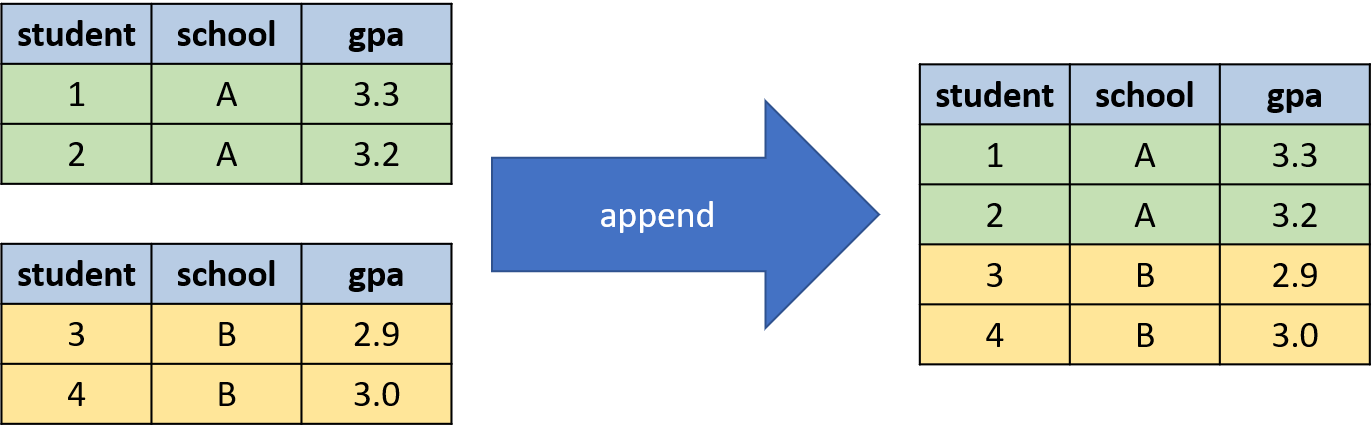
\includegraphics[width=\textwidth]{images/append.png}
\end{center} \pause \bigskip
From the pre class exercise: \texttt{append using person2016}
\end{frame}

\begin{frame}
\frametitle{Merge 1:1 when both tables have same unit of analysis}
\begin{center}
	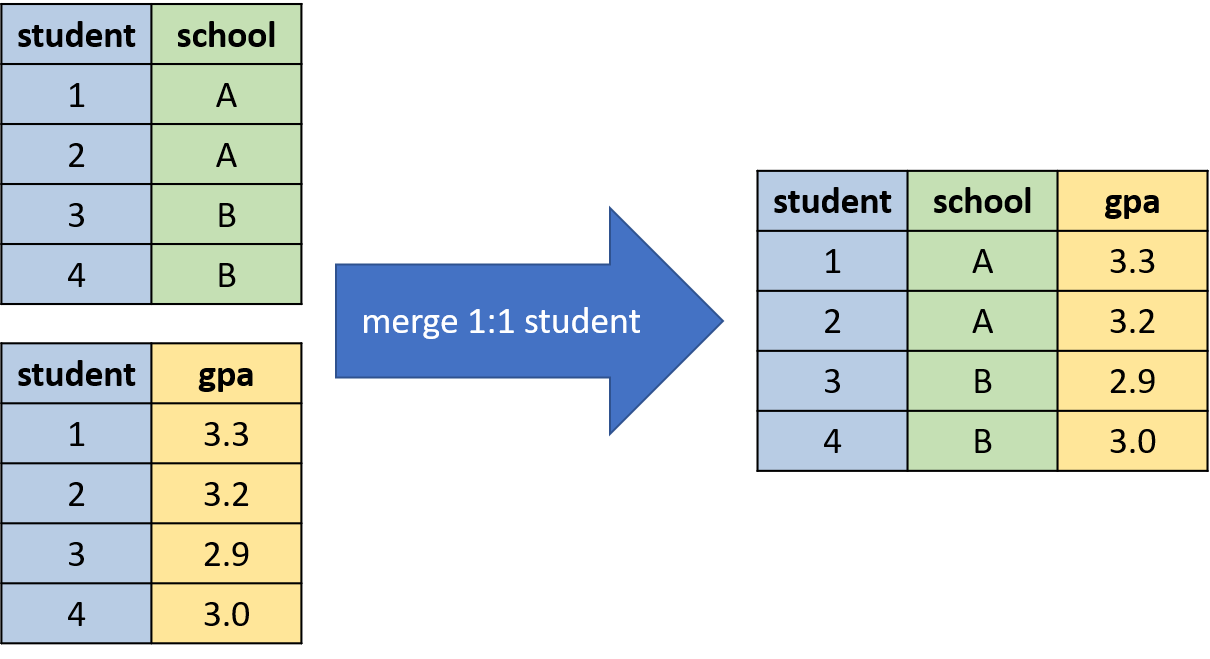
\includegraphics[width=0.9\textwidth]{images/merge_one.png}
\end{center} \pause \bigskip
From the pre class exercise: \\ \texttt{merge 1:1 year id using demographics.dta}
\end{frame}

\begin{frame}
\frametitle{Next, we will generate summary statistics at the year level.}
What is the unit of analysis of class13.dta? \\ \bigskip \pause
\begin{itemize}
	\item[1a.] Sort your data: \pause
	\item[   ] \texttt{sort year id} \pause \bigskip
	\item[1b.] Generate an variable to indicate the first observation in each year: \pause
	\item[   ] \texttt{by year: gen firstob = 1 if \_n == 1} \pause \bigskip 
	\item[1c.] Generate means of \texttt{perwt - female} by year: \pause
	\item[   ] \texttt{by year: egen perwtmean = mean(perwt)}
\end{itemize} \pause \bigskip
Only plot one observation per year by adding: \pause \texttt{if firstob == 1}
\end{frame}

\begin{frame}
\frametitle{Collapse to coarsen the unit of analysis}
\begin{center}
	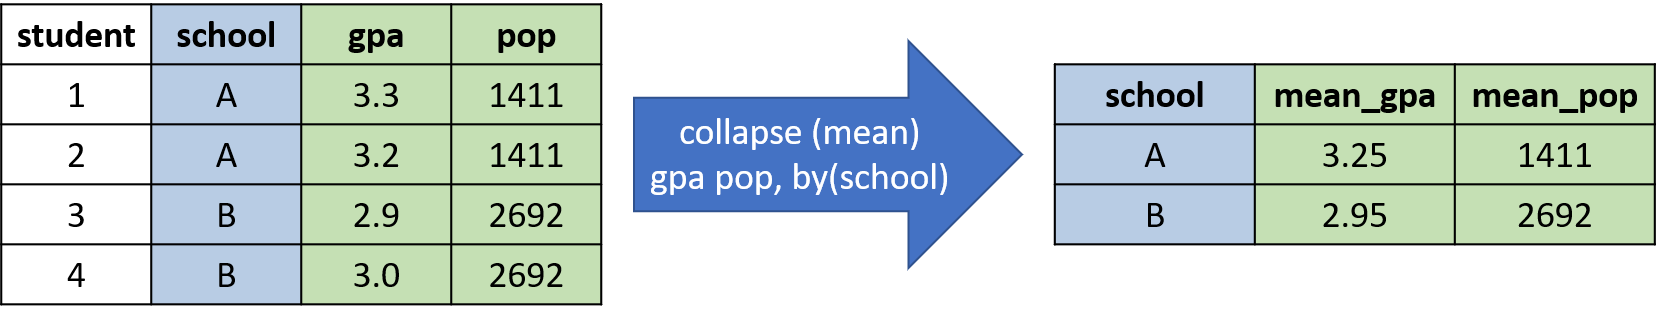
\includegraphics[width=\textwidth]{images/collapse.png}
\end{center}
\end{frame}

\begin{frame}
\frametitle{We can collapse our data to easily calculate summary statistics.}
What is the unit of analysis of class13.dta? \\ \bigskip \pause
\begin{itemize}
	\item[2a.] Collapse the data from person-year to year using weights: 
	\item[   ] \texttt{collapse (mean) perwt - female [aweight = perwt], by(year)} \pause \bigskip
	\item[2b.] Run the code listed to rename your variables appropriately. \pause \bigskip
	\item[2c.] Save this new data frame as class13collapsed.dta: \pause
	\item[   ] \texttt{save class13collapsed, replace} \pause \bigskip 
\end{itemize}
Create your plot and notice that including weights slightly changes the mean (why?). 
\end{frame}

\begin{frame}
\frametitle{Merge m:1 when one table has a coarser unit of analysis}
What is the unit of analysis of each table?
\begin{center}
	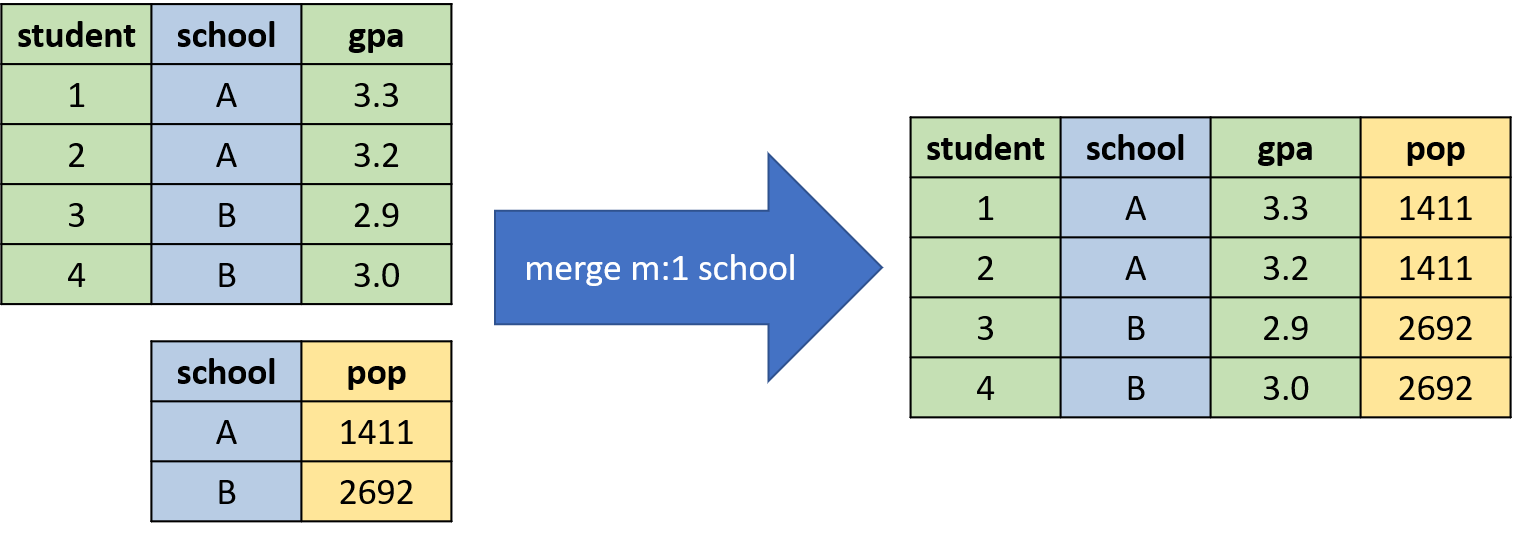
\includegraphics[width=\textwidth]{images/merge_many.png}
\end{center} \pause \bigskip
Your turn! Complete a m:1 merge to complete question 3.
\end{frame}

\begin{frame}
\frametitle{Changing data form: ``long'' vs ``wide''}
Often we have multiple entries of a given variable for the same unit (e.g. multiple GPAs for the same student observed once per quarter). \\ \bigskip
We can present these data as \alert{long} or \alert{wide} and convert between the two using \alert{reshape}.
\begin{center}
	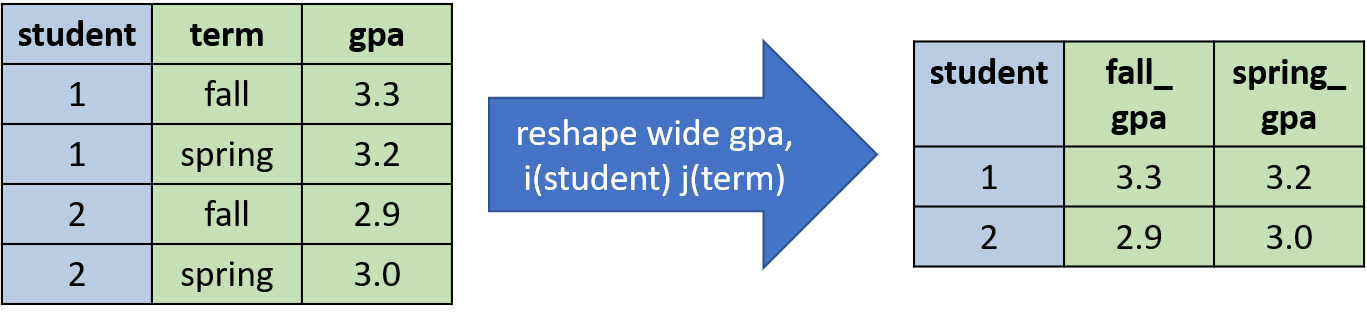
\includegraphics[width=\textwidth]{images/reshape.png}
\end{center} \pause \bigskip
Your turn! Reshape class13.dta to complete question 4.
\end{frame}

\begin{frame}
\frametitle{Here are the commands/operators we covered today:}
\begin{columns}
	\begin{column}{0.5\textwidth}
		\begin{itemize}
			\item \texttt{append}
			\item \texttt{merge 1:1; merge m:1}
			\item \texttt{\_n}
			\item \texttt{collapse}
			\item \texttt{aweight}
			\item \texttt{reshape wide}
			\item \texttt{reshape long}
		\end{itemize}
	\end{column}
	\begin{column}{0.5\textwidth}
	\end{column}
\end{columns}
\end{frame}

\end{document}